\documentclass[10pt, a4paper, twoside]{amsart}

\usepackage[english]{babel}
\usepackage{amsthm,amssymb,amsmath,graphicx}
\usepackage{bbm}
\PassOptionsToPackage{hyphens}{url}\usepackage{hyperref}

\newcommand{\N}{\mathbb{N}}
\newcommand{\Z}{\mathbb{Z}}
\newcommand{\Q}{\mathbb{Q}}
\newcommand{\R}{\mathbb{R}}
\newcommand{\C}{\mathbb{C}}
\newcommand{\D}{\mathbb{D}}
\renewcommand{\a}{\alpha}
\renewcommand{\d}{\delta}
\newcommand{\p}{\partial}
\newcommand{\e}{\epsilon}
\newcommand{\w}{\omega}
\renewcommand{\l}{\lambda}
\newcommand{\vp}{\varphi}
\newcommand{\vn}{\emptyset}
\newcommand{\bs}{\backslash}
\newcommand{\A}{\mathcal{A}}
\newcommand{\F}{\mathcal{F}}
\renewcommand{\P}{\mathcal{P}}
\newcommand{\1}{\mathbbm{1}}
\newcommand{\im}{\textup{im}}
\renewcommand{\p}[2]{\frac{\partial #1}{\partial #2}}%partial
\renewcommand{\a}[1]{\left\lvert #1 \right\rvert}%abs
\renewcommand{\b}[1]{\left( #1 \right)}%brackets
\newcommand{\n}[1]{\left\lVert #1 \right\rVert}%norm

\newtheorem{definition}{Definition}
\newtheorem{lemma}{Lemma}
\newtheorem{theorem}{Theorem}

\newcommand\textbox[1]{
  \parbox{.333\textwidth}{#1}}

\newcommand{\homeworkset}{}
\newcommand{\courseName} {A3.6 Maze Generation}
\newcommand{\firstName}  {Wouter}
\newcommand{\lastName}   {Slegers}
\newcommand{\studId}     {19950825-1957}
\renewcommand{\email}    {wjslegers@gmail.com}

\pagestyle{plain}
\begin{document}
\noindent{\huge\bf \courseName}\\
\noindent\textbox{\sc \firstName~ \lastName \hfill}\textbox{\hfil Uppsala University \hfil}\textbox{\hfill \studId}
\noindent\textbox{\large\sc Report \hfill}\textbox{\hfil \today \hfil}\textbox{\hfill \email}
\bigskip


\section*{Introduction}
I have elected to do project A3.6 and make a maze generation algorithm. I came up with three different algorithms. The first a search algorithm, the second is inspired by random walks and the last one is inspired by generational teaching of AI to play games, which is not very suitable for the purpose but fun to work with!

\subsection*{Practical information}
I use the word maze for any set of fields arranged in a square, with walls around the edges and each field is connected to its horizontal or vertical neighbours either by a 'wall' or an 'opening'. We may speak of fields being connected or not depending on a wall being there. Also I use the words node and field interchangeably.
I set the goal of a 'correct maze' as a maze that has a path of connections from the top left to the bottom right. In the code that is from field \verb+(0, 0)+ to field \verb+(maze.fields - 1, maze.fields - 1)+, where \verb+maze.fields+ is the number of fields of maze. The goal is to create an algorithm that makes such a 'correct maze', preferably with as many walls still standing, one could after all just remove all walls and be done with it, but be left with a rather boring maze.\\

To make writing code as easy as possible I chose Python, as I find it quick and easy to set things up. 
You can find all the Python files in the zip-folder.
I made a 'Maze' class and print it using the 'print()' function of Python to simplify the creating of the graphical part of the program.


\section{Path Through Maze Algorithm}
The idea of the algorithm is to first generate a relatively dense random maze. For example, for each wall there is a $70\%$ chance it becomes a wall and $30\%$ it is left open. Then we use a search algorithm that saves all the nodes it can reach from the starting node in a list called \verb+searched+. Every one of those nodes that is a dead end it also saves in a list called \verb+dead_ends+, a dead end we define as a node with three or more walls around it. If we come across the end node we stop the algorithm. Otherwise we go through the dead ends until we find one that has a wall that leads to a previously unexplored node i.e. the neighbouring node is not in \verb+searched+. We remove the wall and the algorithm repeats the search but starting from the node that we just connected. We can keep the \verb+searched+ and \verb+dead_ends+ lists, the latter minus the newly opened up field, of course. This way we 'search' each node only once and the time the algorithm takes stays limited.

\subsection{Why it works}
The idea is that the algorithm will not stop searching the maze and opening up connections until there is a path that reaches the end ensuring that it gives a correct maze. However, it is possible that there are no suitable dead ends during one of the steps in the algorithm. See the figure below with such an example. On the right is the same maze but with the fields marked 's' for searched or 'd' for searched and a dead end. The guarantee we do have is that if we do not reach the end of the maze with our search there must be a searched node with a neighbour it is not connected to yet. So if we do not find a suitable dead end we take such a searched node to open up a new connection from and start our search from again.
This is necessary to make sure we always end up with a correct maze, but it must be said that the situation does not occur all that often. This, in part we can thank to the fact that we start with a randomized maze.

\begin{figure}
\centering
        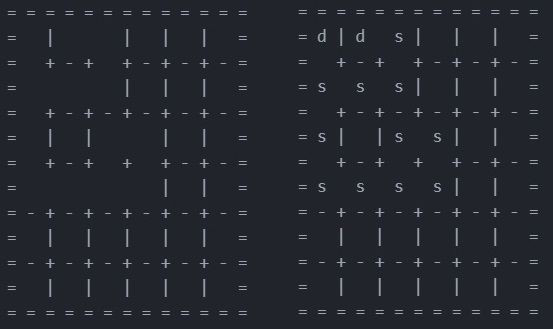
\includegraphics[totalheight=8cm]{nodeadends}
    \caption{Example of a maze without suitable dead ends}
\end{figure}

\subsection{Tweaks to the algorithm}
There are some choices we can make. An important one is the begin density of the maze. Make it too open and there'll already be some paths to the end, and a sparse maze isn't the most interesting. Make it too dense and then there will be whole sections of the maze completely blocked off and never having been searched. The choice of $70\%$ seems to work most of the time.
Furthermore we have a choice of which dead end we open up in each step (or alternatively which searched node we open up) and a choice of which neighbour we open it up to.
I chose to favour opening up dead ends further away from the diagonal line between the beginning and end, to favour more interesting paths, with the following line of code.\\
\verb+dead_ends.sort(reverse=True, key=lambda node: abs(node[0] - node[1]))+\\
After this we take the first suitable dead end we find in the list. For the choice of neighbour we go with a random one. Also if we need to open a searched node instead of searched dead end, it is picked randomly.

\subsection{Notes and performance of the algorithm}
Since in the worst case each field has to be searched we may have to search $n^2$ fields for a square maze of $n$ by $n$. In the worst case each search adds only one node to the list \verb+searched+ and each time we do a sort of \verb+dead_ends+ (which has time complexity $n\log n$) and in the worst case about a third of the field could be dead ends. These situations are thankfully rather unlikely but, long story short, the worst case time complexity is not great. In practicality it is perfectly capable of creating mazes of $50$ by $50$ within seconds (on my PC anyway). Going higher than this may lead to call-stack errors, with too many recursive calls taking place.\\

The algorithm does not open up walls unnecessarily, in the end there will be a unique path to the end. Other nodes that we opened that did not lead to the end make for dead ends, which makes for a more interesting maze.\\

Unfortunately with the random nature of the algorithm it can happen that few nodes get searched (sometimes only around half, often most of them above or most of them below the top-left-to-bottom-right diagonal), 
leaving the rest of the maze as it was randomly initialised. Thankfully it seems to, most often, search most of the maze and return a relatively interesting maze.\\

To run the generation just execute \verb+PathThroughMaze.py+. The call\\ \verb+maze = create_maze_ptrm(12, 0.7, True)+ creates a maze of 12 by 12, with starting density of $70\%$ and True indicates it will print each step in between. When printing the maze you can use \verb+maze.print(False)+. False indicating that you do not want to leave the fields empty. With True it also print the fields, which during the algorithm get marked with 's' if they've been searched, which in turn can get overridden by 'd' for dead ends or 'O' if it is a node that has been opened.


\section{Self-avoiding random walk}
The idea of this algorithm is to start a self-avoiding random walk from the beginning of the maze, leaving a path of connections through an initially fully walled in maze. Whenever it can make no further steps we repeat, but start from a previously visited node with a previously unvisited neighbour. We don't stop until  every node has been visited. This results in a fully connected maze, which ensures a path from beginning to end.

\subsection{Tweaks to the algorithm}
I have added a \verb+CHANCE_STRAIGHT+ variable in the code. If set to $0$ the walk will be truly random. If set to, for example, $0.3$, then, in each step, there is a $30\%$ chance we first check the node that is in the same direction as the previous step we set, and move to that one next if it is a suitable field. This creates longer corridors in the maze. This means I send a direction variable in each function call. Setting it to $-1$ means we don't use it. 

\subsection*{Notes on the algorithm}
To run the generation just execute \verb+Walker.py+. The call\\ \verb+maze = create_maze_walker(15)+ creates a maze of $15$ by $15$. Whether we print the steps in between is this time done with the boolean \verb+PRINTING_STEPS+, sorry for the inconsistency.\\

IMPORTANT NOTE: This algorithm can not generate mazes larger than $32$ by $32$. Since each step it sets means a recursive call we would get a call-stack error. We could have programmed the algorithm to only do a recursive call every time it starts a new path, and save visited nodes and the current position and direction in a different way to avoid the problem and create bigger mazes.

\section{Generational learning}



\end{document}